\section{LEGENDRE Associated Legendre Polynomial}

\subsection{Usage}

Computes the associated Legendre function of degree n. 
\begin{verbatim}
  y = legendre(n,x)
\end{verbatim}
where \verb|x| is either a \verb|float| or \verb|double| array in range \verb|[-1,1]|, \verb|n| is integer scalar.  The output
vector \verb|y| is the same size (and type) as \verb|x|.
\subsection{Example}

Here is a plot of the \verb|legendre| function over the range \verb|[-1,1]|.
\begin{verbatim}
--> x = linspace(-1,1,30);
--> y = legendre(4,x);
--> plot(x,y); xlabel('x'); ylabel('legendre(4,x)');
\end{verbatim}
which results in the following plot.


\centerline{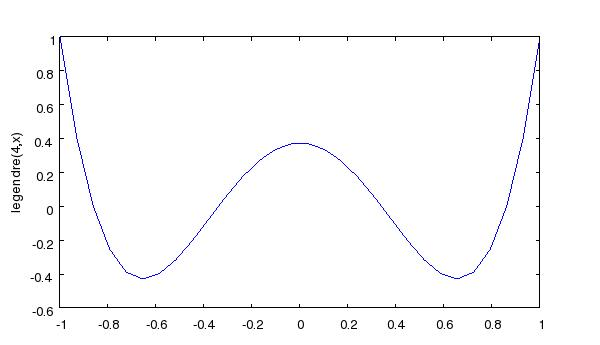
\includegraphics[width=8cm]{legendre}}

